
\Chapter{Basic element types}%\index{element types}
\label{elements}

The basic element types which ElmerSolver can handle are
the linear and quadratic elements in one, two, and three dimensions:
\begin{itemize}
\item linear (element type code 202) and quadratic (203) elements in one dimension
\item linear (303) and quadratic (306) triangles with three and six nodes, respectively; 
see Figure~\ref{triangles}
\begin{figure}[h]
\centerline{ \includegraphics[width=2in]{3node_tri.ps}\ \ \ \ \includegraphics[width=2in]{6node_tri.ps} }
\caption{The linear (303) and quadratic (306) triangular elements.}
\label{triangles}
\end{figure}
\item bilinear (404) and quadratic (408,409) quadrilaterals with four, eight, and nine nodes, respectively;  
see Figure~\ref{quads}
\begin{figure}[h]
\centerline{ \includegraphics[width=2in]{4node_quad.ps}\ \ \ \ \includegraphics[width=2in]{8node_quad.ps} }
\caption{The four-node (404) and  eight-node (408) quadrilateral elements.}
\label{quads}
\end{figure}
\item linear (504) and quadratic (510) tetrahedrons with four and ten nodes, respectively; 
see Figure~\ref{tetras}
\begin{figure}[h]
\centerline{ \includegraphics[width=2in]{4node_tetra.ps}\ \ \ \ \includegraphics[width=2in]{10node_tetra.ps} }
\caption{The linear (504) and quadratic (510) tetrahedron elements.}
\label{tetras}
\end{figure}
\item  trilinear (808) and
quadratic (820,827) bricks  with 8, 20, and 27 nodal points, respectively; see Figure~\ref{hexas}.
\begin{figure}[h]
\centerline{ \includegraphics[width=2in]{8node_brick.ps}}
\centerline{ \includegraphics[width=2in]{20node_brick.ps}}
 \caption{The 8-node (808) and 20-node (820) brick elements.}
\label{hexas}
\end{figure}
\end{itemize}

%Further element types belonging to these basic topologies may be added to the program by
%editing element type definition file without touching the solver code nor compiling or
%linking the program. How to create a mesh using these element types is a separate question. 

%The definition file is read in when the solver code is initialized and a basis function matrix is
%formed for every element type defined. The rest of the FEM code (computing local and global
%derivates, integration of elements) is then basically independent of the element type.
